\subsection{Another Try to Solving the DNA Detection Problem}
Besides the greedy algorithm based on huffman coding, we can also use the GBSC to solve the DNA detection problem.

% \begin{enumerate}
%     \item First we choose a continuous stretch of DNA, in which the sum of probabilities of exons is most close to 0.5.
%     \item Second we examine whether the target exon is in the stretch we found in the first step.
%     \item If the target is in the stretch, we can set the probabilities of exons outside the stretch to 0 and normalize the probabilities of other exons to make the sum of their probabilities equal to 1; if the target is not in the stretch, we set the the probabilities of exons in the stretch to 0 and normalize the probabilities of other exons to make the sum of their probabilities equal to 1
%     \item Repeat the above steps until there is only one exon whose probability is not equal to 0 and it is the target exon.
% \end{enumerate}
We compared the output and time cost of the two algorithms by using the same random seed to generate random sequences (assuming probability at every point is iid) of different lengths and using the two algorithms to compute the expected number of detections respectively. We generated 100 sequences for each length to reduce random error. Here are the results.

The average time cost for two algorithm is shown in Fig.\ref{fig:runningtime}.
\begin{figure}[H]
    \centering
    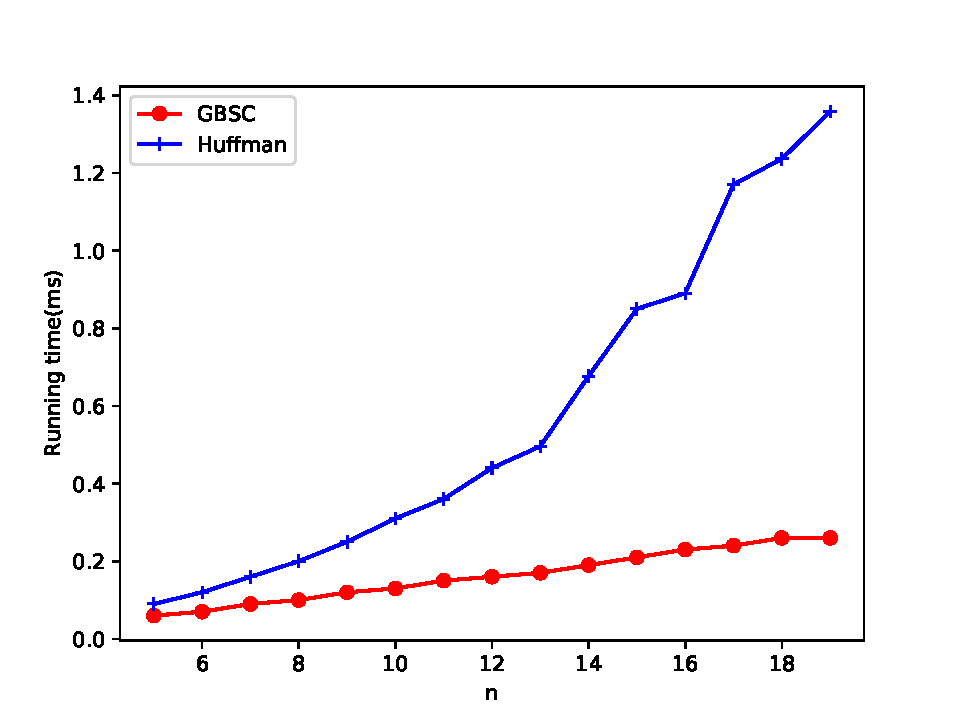
\includegraphics[width=0.55\textwidth]{figure/BHTime.pdf}
    \caption{Running time of the two algorithms.}
    \label{fig:runningtime}
\end{figure}

It can be seen from the figures that the time complexity of GBSC is nearly linear, while the time complexity of the Huffman-based algorithm is not. The GBSC-based algorithm runs much faster than the Huffman-based algorithm algorithm. Besides, the the Huffman-based algorithm is not robust, and would take quite a long time to give an output when initial data is not very ideal. For example, one of the randomly generated distributions with size 36 took it took about 30 seconds for the Huffman-based algorithm to calculate the result, while most other distributions usually took about 10ms. In comparison, the GBSC reliably gave results in a relatively short time.
%\vspace{1ex}

The expected lengths calculated by two algorithm are shown in Fig.\ref{fig:GBSCvsHuffman}.
\begin{figure}[H]
    \centering
    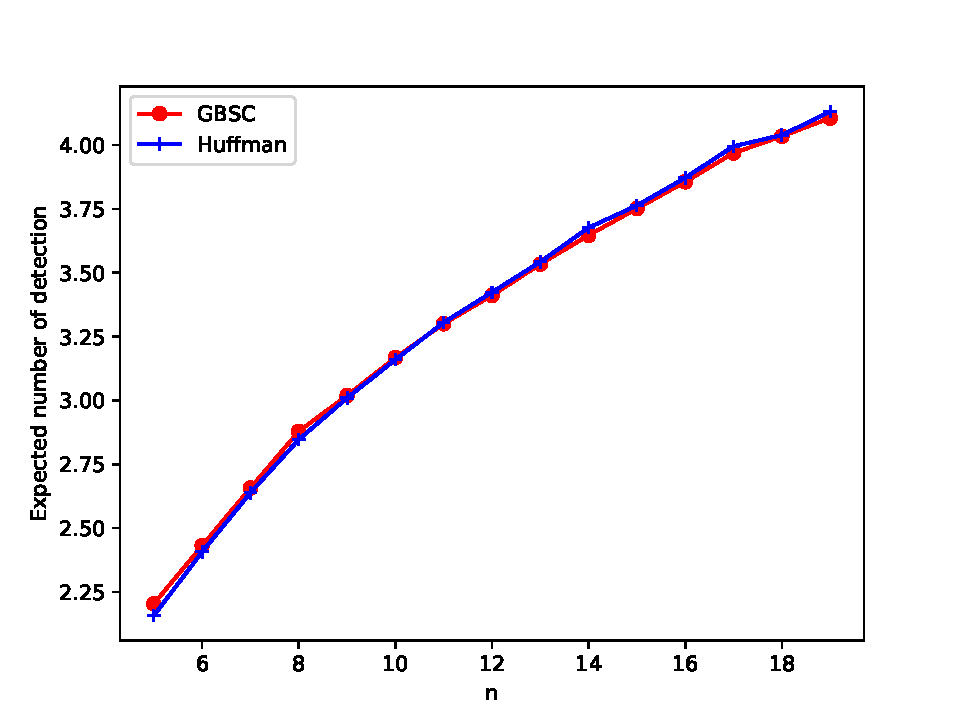
\includegraphics[width=0.55\textwidth]{figure/BHLength.pdf}
    \caption{Expected number of detections calculated by the two algorithms.}
     \label{fig:GBSCvsHuffman}
\end{figure}
It is easy to see that the two figures are very similar, which means that the outputs of two algorithm in our experiment are almost the same.

